% #############################################################################
% This is Chapter 1
% !TEX root = ../main.tex
% #############################################################################
% Change the Name of the Chapter i the following line
\fancychapter{Introduction}
\cleardoublepage
% The following line allows to ref this chapter
\label{chap:intro}

	The act of making something as fully perfect, functional or effective as possible is a behavior that is constantly sought by us, Humans, in a process known as optimization ~\cite{MerriamWebster2017OptimizationDefinition}. Intuitively, through optimization one aims to improve a system in terms of different quantitative measurable aspects. Although usually striving to fully optimize these systems, i.e., to obtain \textit{perfect} systems, it is often the case that finding a better one or a near-optimal system suffices.

	Generally, optimization processes are composed of two main parts: (1) the model of the system to be optimized and (2) the algorithm responsible for finding the optima. Conceptually, the model is a description of the system that is comprised of (a) variables or unknowns, i.e., representations of the system's characteristics, (b) objectives or criteria, i.e., quantitative measures of the system's performance and that are usually functions of the system's variables, and, optionally, (c) constraints, i.e., system's conditions that have to be satisfied to guarantee the system's feasibility~\cite{Nocedal2011NumericalOptimization}. Subsequent to model definition, we reach the second part of optimization processes, that is, to search among the set of possible solutions for the optimal ones. The strategy used to search the solution space is the responsibility of optimization algorithms, which enclose a detailed description of the steps necessary to attain optimal solutions. The optimal solutions depend on the values of the model's objectives, and the search directions depend on whether they should be maximized or minimized. 
	
	In the mathematical sense of optimization, these processes can be classified differently depending on the numerous alternatives for representing models or on the strategy underlying the search for optimal solutions. Concretely, models representations may differ in the variables' type, the presence of absence or constraints, the number and nature of objective functions, among others, whereas search strategies might explore vaster or narrower regions of the solution space. Although we introduce four of these classifications, we refer the interested reader to \cite{Nocedal2011NumericalOptimization,Nemhauser1988} for a more comprehensive treatments of these subjects. We selected four classifications due to their relevance and their ubiquitous in optimization problems.
	
	The first classification differentiates continuous and discrete optimization problems depending on the variables' types. Continuous optimization refers to problems defined uniquely by continuous variables and, therefore, characterized by an infinite solution space, whereas discrete optimization refers to problems for which some or all their variables are discrete, hence yielding a finite solution space. In continuous optimization, the smoothness of functions make it possible to reason about the behavior of all points close to $x$ and, consequently, to solve these problems more easily, whilst the commonly present irregularities of discrete optimization functions do not, in general, allow to draw any information about the behavior of points close to $x$. Moreover, the discrete classification encloses finer classes, such as integer optimization or combinatorial optimization~\cite{Nemhauser1988}. 
	
	The second classification is related to the absence or presence of constraints on the variables. Unconstrained optimization problems result from many practical applications and have no restrictions on the values of the variables. Contrastingly, constrained optimization problems usually emerge from systems for which constraints are crucial (e.g., economy problem, imposing cargo constraints) and, therefore, incorporate such constraints into the problem's definition ~\cite{Nocedal2011NumericalOptimization}. Variables can be conditioned using hard or soft constraints. The former sets conditions for the variables that must be satisfied, i.e., to vary within simple bounds (e.g.: $-1<x<1$) and to relate to other variables in certain ways (e.g.: $\sum_{i} x_i$), whereas the latter sets penalties for the variables whose value violates the condition. Constrained optimization are often converted to unconstrained optimization problems by replacing hard constraints by soft constraints, i.e., by adding penalization terms in the objective function to discourage the violation of constraints. 
	
	The third classification distinguishes optimization problems in terms of the aim of the search, particularly, whether it is a global or a local search. In local optimization, the search process strives to find a solution that is locally optimal, i.e., for which its value is better than all other points in its vicinity. The points that satisfy the previous property are known as local optima. On the other hand, global optimization problems strive to find the globally optimal solutions, i.e., the best of all the local optima.

	The fourth, and final, dichotomy herein discussed is with respect to the number of objectives to optimize, which are distinguished in single-objective and multi-objective optimization. Indeed, optimization is frequently required to address problems involving more than one objective. For example, people often face decisions involving two or more conflicting objectives, either to effectively manage resources, or just to ponder several factors associated with certain decisions (e.g.: purchase a house). As opposed to simpler single-objective optimization problems, which focus on the optimization of one objective, these processes are examples of \ac{MOO} problems, as they attempt to simultaneously optimize multiple conflicting objectives.%A simple example is the act of purchasing something, e.g., a computer or a car. In these settings, people often ponder different aspects to determine the best choice, i.e., to optimize its decision. In general, when looking for a computer, one is usually interested in minimizing the price of the computer, while maximizing the processing speed, the RAM's capacity and speed, the storage's capacity and speed, and the battery autonomy. However, while some aspects are independent of each other, e.g., processing speed and RAM capacity, other aspects are conflicting and preclude the simultaneous satisfaction of all the objectives, e.g., the higher the speed of processing units, storage or RAMs, the higher the price, and the worse the battery's autonomy.
	 
	% Although the previous example presents a simplified version of a real decision process, it evidences the large complexity that day-to-day decision processes might enclose. As opposed to simpler single-objective optimization problems, which focus on the optimization of one objective, this example is a \ac{MOO} problem, which attempts to simultaneously optimize multiple conflicting objectives.
	
	The application of optimization goes beyond day-to-day life decisions, also having a paramount impact on decisions involved in fields like economy, science, engineering, among others. As a case in point, optimization yields a great potential to architectural practices, for it directly impacts the building industry: optimization enables the reduction of the economic and ecological footprint of the building sector through the finding of more efficient building variants, prior to their construction. Given its importance to the world's sustainability and economy, this thesis focus on the application of optimization processes to enhance the architectural practice. The following sections provide an overview of the involvement and the evolution of these processes in the architectural field. We end this chapter by highlighting our research goals and by outlining this thesis structure.

%% #############################################################################
\section{From Design to Optimized Design}
	
	The usefulness of optimization goes beyond architectural design applications, benefiting other engineering fields, like Mechanics and Electronics, through the optimization of components and circuits designs. 
	
	In the architectural practice, optimization has been gaining relevance for the past few years~\cite{Cichocka2017SURVEY}, especially due to the impact of building construction and building maintenance in the economy and environment. For this reason, designers are shifting from a pure aesthetically-based to performance-based design, where buildings are being optimized to achieve the best possible values regarding different aspects of their design, such as thermal comfort, energy consumption, lighting comfort, structural behavior, cost, among others.

	This has only been possible due to the technological improvements in the architectural practice over the last few decades. The adoption of computer science techniques was responsible for the dissemination of digital modelling tools, which allowed for more accurate and efficient design of highly complex buildings. These tools enabled a shift from traditional paper-based approaches to more computerized ones, such as \ac{CAD} and \ac{BIM} applications, where changes to designs are trivial and do not require manually erasing and redrawing parts of the original design~\cite{Ferreira2015GD}.~\Cref{fig:traditionaldesign} illustrates the general view of this computer-aided design process, as well as an example of a 3D modeling tool. The architect interacts directly with these modeling tools to incrementally realize his design ideas.
	
\begin{figure*}[htbp]
\centering
\subfigure[]{%
\label{fig:traditionaldesign-a}%

\includegraphics[width=0.38\textwidth]{./Images/Introduction/TraditionalArchitecturalDesign.png}}%
\hfill
\subfigure[]{%
\label{fig:traditionaldesign-b}%
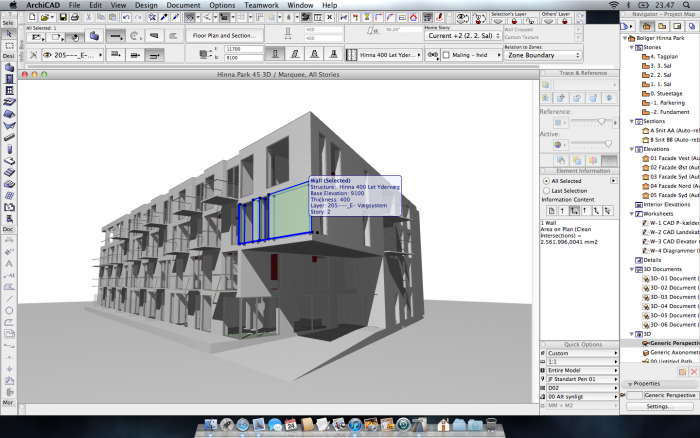
\includegraphics[width=0.48\textwidth]{./Images/Introduction/Example3DModellingTool_1.png}}%

\caption[General views of Traditional Design Approaches]{(a) Simplification of a computer-aided design workflow (b) Building design example in a 3D modeling tool. Image retrieved from~\cite{3DMODELTOOL}}
\label{fig:traditionaldesign}
\end{figure*}

Shortly after, the development of computer-based simulation tools enabled designers to simulate the behavior of building designs regarding specific criteria, i.e., to get a measurement of its performance~\cite{Malkawi2005}. Through this process, called \ac{BPS}, designers could easily validate whether their building's performance satisfied the efficiency requirements and, ultimately, optimize their design by iteratively generating multiple variations of the same design, assessing their performance, and selecting the better ones. Albeit being very primitive, architects now had the elementary mechanisms required for optimizing their building's designs, which spurred a new performance-based approach.

% #############################################################################
\subsection{Building Performance Optimization}

	\ac{BPO}, a simulation-based optimization approach, treats the results produced by the simulation tool as the functions to optimize. Although invariably suffering from some degree of imprecision and inaccuracy, using these simulations it becomes possible to estimate the performance of complex designs. Particularly, these estimates are beneficial in designs for which analytical solutions are often very difficult or even impossible to derive~\cite{Kolda2003}. In these cases, the objective function, i.e., the function to optimize, is derived from the simulations' results. These functions have a domain which corresponds to the range of acceptable designs, as specified by the architect.

	A known drawback of simulation-based approaches is the time required to achieve reasonable results for complex systems~\cite{Law1991} which is associated with different aspects of the problem, namely: (1) its \textbf{domain} which, depending on the nature of the problem, might use different methodologies to produce the corresponding estimates (e.g., thermal \textit{versus} structural); (2) its \textbf{intrinsic structure} which, depending on the attributes and relations of the system, might lead either to simpler or to more complicated computations (e.g., skyscraper \textit{versus} a small house); and (3) its \textbf{analytical model}, which has the essential properties of the system we are trying to simulate and that will be used as input to the simulation tool. Generally, the domain and structure do not change for the same problem, albeit there are numerous ways to produce multiple analytical models. Depending on the level of detail of the analytical model (e.g., using a single plane \textit{versus} a mesh to represent a non-planar surface), both the computational time and the result of the simulation might change. 

	In architecture, the generation of each analytical model is a time-consuming and complex task. On the one hand, it is often necessary to generate multiple models of the same design because of the simulation tools' specificity, i.e., in order to evaluate a design, each simulation tool requires a specialized model of the same design. On the other hand, simulation tools often yield time-consuming processes, where a single simulation can take up to seconds, minutes, hours, days, or even weeks to complete. 
	
	In addition to the simulations' specificity and complexity, architectural designs are inherently complex, thus leading to less predictable objective functions, for which mathematical forms are difficult to formulate~\cite{Machairas2014}. For this reason, information about the derivatives of such functions cannot be extracted, and methods depending on function derivatives cannot be used to address architectural optimization problems. Particularly, classical gradient-based optimization methods cannot be used because they exploit the function's derivatives. Instead, other methods that do not rely on the existence of an explicit mathematical form should be used, i.e., methods that treat the optimization functions as black-boxes, relying uniquely on the outputs of numerical simulations.
	
% Motivation for other design alternatives
	Despite the flexibility provided by \ac{CAD} and \ac{BIM} tools, architects often face difficulties when modeling complex geometry. A \ac{BPO} methodology requires the experimentation of different design variations, which implies spending a large amount of time to manually make changes to the design. Since an optimization process requires evaluating several variations of the same design, the manual execution of the required changes implies a lot of effort, hence making the whole optimization process unviable.
	
% #############################################################################
\subsection{Algorithmic Design}

% Introduction to AD, way of overcoming limitations of manual approaches
	An approach capable of creating forms through algorithms is crucial for overcoming the aforementioned limitations. An example of such approach is \ac{AD}~\cite{Branco2017AD} and \Cref{fig:algorithmicdesign} illustrates a simplified view of its application in a design workflow. In this approach, the architect entails an algorithmic description of the intended design. After elaborating the algorithm, executing it will automatically generate the corresponding 3D model in a \ac{CAD} or \ac{BIM} tool. Algorithmic approaches are inherently parametric, thus enabling the generation of different variations of the same design by making simple modifications to the values of the parameters~\cite{Leitao2014GD}. 
	
\begin{figure}[htbp]
\centering

\includegraphics[width=0.70\textwidth]{./Images/Introduction/AlgorithmicArchitecturalDesign.png}
\caption[General view of the Algorithmic Design Approach]{Algorithmic-based design workflow}
\label{fig:algorithmicdesign}
\end{figure}
	
	As an example, consider the algorithmic design of Astana's National Library from the Bjarke Ingels Group (BIG) architects, illustrated in~\Cref{fig:astana-a}. Initially, the architect selects an \ac{AD} tool providing the necessary design primitives. Then, he uses those primitives to create a computational program enclosing the relative relations among the different design elements, so that when a modification occurs in one element, that same modification is propagated throughout that element's dependencies. In the end, the architect creates a procedure responsible for creating the whole design, which when executed will produce the corresponding Astana 3D model. Because the Astana's design resembles a \textit{möbius} strip, define the procedure in terms of two parameters: the radius, defining the whole width of the design, and the number of twists of the strip. Now, he is able to easily generate different variations of the Astana by invoking the procedure with different values for these parameters. \Cref{fig:astana} illustrates the original design, two design variations, where the radius and the number of turns in the design are increased, respectively. 
	
\begin{figure*}[htbp]
\centering
\subfigure[]{%
\label{fig:astana-a}%
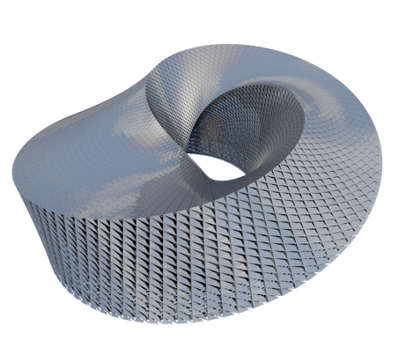
\includegraphics[width=0.32\textwidth]{./Images/Astana/Astana1.png}}%
\hfill
\subfigure[]{%
\label{fig:astana-b}%
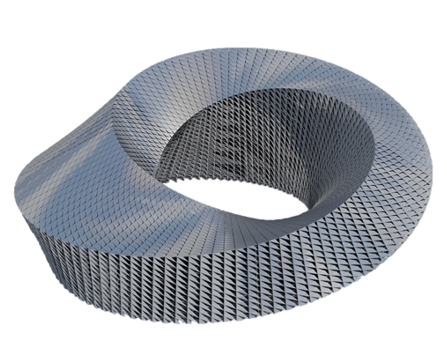
\includegraphics[width=0.33\textwidth]{./Images/Astana/Astana2.png}}%
\hfill
\subfigure[]{%
\label{fig:astana-c}%
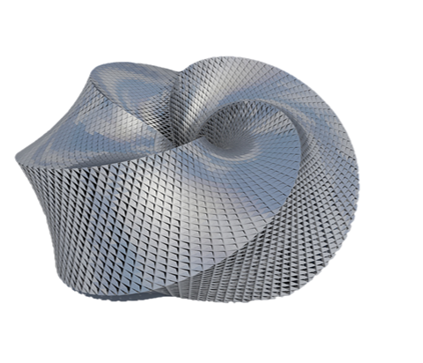
\includegraphics[width=0.33\textwidth]{./Images/Astana/Astana3.png}}%

\caption[Design variations of the Astana's National Library]{Astana's National Library Design variations: (a) Original (b) Larger diameter (c) Two \textit{möbius} twists}
\label{fig:astana}
\end{figure*}

% Advantages over Manual approaches & Disadvantages
Only recently has the algorithmic paradigm begun to settle in the architectural practice. The requirement for programming knowledge is often an obstacle to the adoption of these approaches, since it requires larger initial investments for architects to learn how to program. Despite these investments, the benefits obtained with algorithmic approaches surpass the ones obtained when using \ac{CAD} or \ac{BIM} tools directly for the design of complex buildings. Particularly, initial investments can be quickly recovered when the need for the incorporation of changes arises or when it becomes necessary to experiment different design variations~\cite{Leitao2014GD}. This is especially important when facing design processes characterized by continuously changing constraints and requirements of the design. In these scenarios, a manual-based approach requires to constantly change the design by hand, thus incurring in a dreadful and tiresome process, whereas an algorithmic approach enables the effortlessly generation of a broader range of design solutions, as well as the easy modification of the algorithmic model to comply with new requirements. As a result, with algorithmic approaches, architects are able to explore larger regions of the design solution space, as well as to explore innovative solutions which were not previous considered due to their time and effort complexity~\cite{Leitao2014GD}.

Another benefit of the \ac{AD} approach is the ease of maintenance of the models involved in building design. In fact, since \ac{AD} usually requires a single model of the design, the algorithmic model, it is easier to maintain in scenarios where changes are frequent. On the other hand, manual-based-approaches often involve the creation and maintenance of multiple models of the same design (e.g., analytical models, 3D models), which quickly becomes hard and tiresome to maintain.

% Conclusion
The appearance of \ac{AD} was crucial for the automation of optimization processes as it enables the automated generation of multiple designs by simply changing the values of the design's algorithmic model. However, to optimize such designs, it is necessary to create the analytical models, which can be very dissimilar to the 3D models produced by the \ac{AD} tool. Therefore, to evaluate the 3D models produced by the \ac{AD} tool, the architect must manually generate the corresponding analytical models. Particularly, for complex buildings, this task requires large time and effort investments, which makes most optimization processes impracticable.

% #############################################################################
\subsection{Algorithmic Analysis}

% Motivação p/ passar de AD p/ AA.
Faster and broader design space exploration prompted the creation of increasingly complex building designs, which became less predictable with respect to different aspects~\cite{Branco2017AD}, such as thermal, lighting, acoustics, among others. Moreover, recent requirements for efficient and sustainable buildings led to the demand for buildings that not only are well-designed, but also exhibit a good performance at those aspects.
	
	% Motivar necessidade de ferramentas de tradução de modelos 
	Nowadays, most of the available simulation-based analysis tools are single-domain toolsets, each analysing different parameters within their domain~\cite{Malkawi2005}, i.e., while a lighting analysis tool measures daylight and glare coefficients, an energy simulation tool measures other coefficients related to thermal, energy consumption, and \ac{HVAC} systems. Unfortunately, this often implies the production of different analytical models for the corresponding simulation tools. Moreover, the 3D models produced by 3D modeling tools are generally dissimilar to the specialized models required by each analytical tool. To evaluate the design performance on different domains (e.g., lighting, energetic, structural), the corresponding analytical models have to be produced either by hand, or through translation processes that convert generic 3D models into specialized models required for analysis.

	% Motivar processos automáticos para tradução 
	Currently available techniques for the production of analytical models exhibit a few limitations, including: (1) hand-made analytical models, which might be a more faithful representation of the original model but they require a considerable amount of effort to create; (2) despite the existence of tools that attempt to convert a 3D model into the corresponding analytical model, this conversion is frequently fragile and can cause errors or loss of information; (3) ideally, the results of the analysis would be used to guide changes in the original design, but these changes require additional time and effort to implement, as does redoing the analysis to confirm the improvements. For this reason performance analyses are typically postponed to later stages of the design process, only to verify the fulfillment of the performance requirements.

	To overcome the time and effort limitations associated with the production of analytical models, one can exploit the ideas of algorithmic approaches to automatically generate the necessary analytical models from an algorithmic description. \ac{AA} is an extension to the \ac{AD} approach that besides enabling the automatic generation of analytical models from a design's algorithmic model, also automates the setup of the analysis tool and the collection of its results~\cite{Aguiar2017}. Following this approach, in an \ac{AD} tool, the architect creates the algorithmic model that describes his design's intents and then changes its configurations as to reflect the analysis tool to use, for example, by changing the values of the configuration parameters. \Cref{fig:algorithmicanalysis} illustrates the \ac{AD} and \ac{AA} design workflow, as well as examples of the Astana's National Library models produced for each tool. Note that, even though the abstract description of the design is the same for 3D and analytical models, the produced models can be very different, e.g., a truss is represented as a graph of nodes and edges when submitted for structural analysis, whereas for lighting analysis the truss is represented by its surfaces, and, in the 3D model, the truss is represented by a set of masses representing its bars and nodes.

\begin{figure}[htbp]
\centering
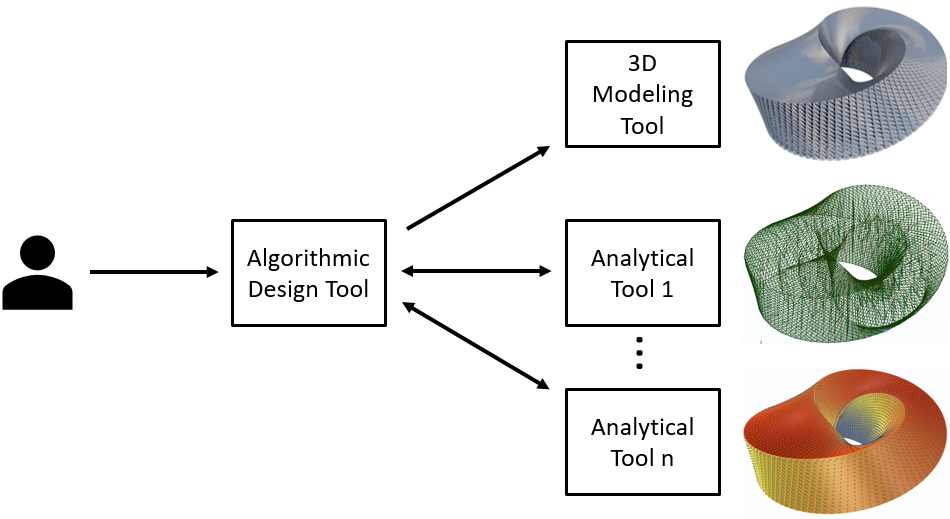
\includegraphics[width=1\textwidth]{./Images/Introduction/AlgorithmicDesignAndAnalysis_w_models2.png}
\caption[General view of the Algorithmic Design and Analysis design approach]{Algorithmic Design and Analysis design workflow with examples of the Astana's National Library design and analytical models: (top) 3D model; (center) Robot's structural analysis model; (bottom) Radiance's pos-radiation analysis model.}
\label{fig:algorithmicanalysis}
\end{figure}		
	
	The \ac{AA} approach is able to enhance performance-based design approaches, as it provides means to effortlessly perform analysis throughout the whole design process, instead of just at final stages. Depending on the performance requirements, architects might need to use different analysis tools: (1) for daylight analysis, Daysim and Radiance are very popular among the community, (2) for energy simulations, EnergyPlus, TRNSYS and DOE-2 are widely used~\cite{Nguyen2014}, (3) for structural analysis, Robot Structural analysis is a well-known reputed tool, and (4) Olive Tree Lab and Pachyderm Acoustical Simulation are examples of good acoustic analysis tools.%~\cite{Branco2017AD}. 
	
	The \ac{AA} approach was also very important to allow the automation of optimization processes, as it abstracted the production of the analytical model, removing the need for direct human intervention and reducing the errors and information loss. Additionally, together with \ac{AD}, it provides the mechanisms to quickly update a design, to generate the corresponding analytical model, to automatically evaluate the design in an analytical tool, and, finally, to collect the results and use them to guide the search for optimal solutions. Despite being possible to automate optimization processes, in order to do so, the architect must define a script entailing an optimization algorithm every time he intends to attain better designs. Besides lacking enough knowledge or expertise about optimization algorithms themselves, in order to entail one, architects would have to either create their own algorithm, or they would have to use one available in some optimization framework. Moreover, because of the efforts associated with the implementation of the optimization algorithm, architects are tempted to adopt the same algorithm to optimize every design, thus instilling performance impacts in the overall optimization time. Among other obstacles, the large time and investment efforts, as well as the lack of knowledge, are often main setbacks to the application of optimization processes in architectural design contexts. 
	
	Despite all the obstacles, optimization prevailed and different approaches have spawned into the architectural practice. During this time, 
	multiple surveys have identified the difficulties and the advantages of each approach, which enabled the development of optimization tools more targeted to architects needs. In the following section, we briefly mention some of these approaches and we emphasize the key points of optimization processes in architecture.
	
% #############################################################################
\subsection{Architectural Optimization Workflow}
	
	In architecture, design optimization might be approached differently. In the past, most optimization processes were comprised of different frameworks, which often had to be integrated with each other. Architects often attempted to integrate existing mathematical optimization and visualization frameworks within their workflow. Due to the tools' specificity, their integration was often an obstacle to the optimization process itself. More recently, the emergence of visual parametric approaches, such as Grasshopper, Dynamo~\cite{GRASSHOPPER,DYNAMOBIM}, among others, coupled with the growing consciousness of both the limitations and the benefits of optimization in building design, have led to the development of ready-to-use optimization toolsets (e.g., Galapagos, Goat, Octopus, Opossum). However, despite enabling the optimization of several designs, visual parametric tools are known to scale poorly with the complexity of the design~\cite{Heijden2015}, thus diminishing and restricting its optimization capabilities. 
	
	On the other hand, textual algorithmic approaches are known to scale well with designs' complexity. In addition to its scalability benefits, its growing popularity among building design practitioners~\cite{Kestelier2013}, its models' flexibility, as well as its capacity to automate optimization processes allow the development of more robust and complete optimization tools. To successfully take advantage of such a tool, an \ac{AD}-based design workflow optimization methodology must be followed. In this approach, the architect idealizes a design which he ought to produce in the corresponding \ac{AD} tool. For this purpose, he creates the computational program, defining the parameters that represent the degrees of freedom in the design, i.e., the parameters which he is willing to manipulate in order to achieve more efficient designs. After the conception of the design's algorithmic model and, provided the values for the parameters, the \ac{AD} tool generates 3D or analytical models for visualization and performance analysis purposes, respectively. Optionally, the architect may decide to optimize his design according to some particular aspects, potentially leading to the exploration of design solutions that were not previously considered. In that case, the optimization algorithm explores different design candidates, using the results produced by simulation tools as the functions to optimize. The execution of the optimization algorithm then yields optimal (or near optimal) design solutions.
	
	Considering the previous view of an algorithmic-based design workflow, we identify four key dimensions in an optimization process:
	
% ------- BEGIN \ --------
\begin{enumerate}
% ANALYTICAL MODELS
\item \textbf{Analytical models}: when the optimization algorithm specifies a candidate design, i.e., a concrete configuration for the parameters of the model, analytical models are automatically generated by the \ac{AD} tool. These models are then used as input for the corresponding analytical tools. These models can be improved, either through simplification of the analytical models, or by enriching them with context information. The former enables the simplification of the analysis itself and potentially reduces the simulation time, by providing an equivalent but simpler model to the tool, whilst the latter enables the attainment of a more detailed and realistic simulation, which is not always possible due to limitations in the \ac{AD} tool. 

% OPTIMIZATION ALGORITHM
\item \textbf{Optimization algorithms}: the algorithms that explore the design space in the quest for optimal (or near optimal) solutions. These algorithms use the results obtained from performance analysis of different design variations as the functions to optimize, i.e., as objective functions. Generally, the algorithm uses these inferred functions to guide the search for optimal solutions. The time complexity of the algorithm is typically dependent on the number of function evaluations. In architectural design, these functions entail time-intensive simulations, thus instilling optimization processes that may take minutes, hours, days, or even weeks to complete.

% EXPLAINABILITY / INTELLIGIBILITY OF RESULTS
\item \textbf{Intelligibility of Results}: Cichocka et al. identify the need for intelligibility of the optimization processes within the architectural community \cite{Cichocka2017SURVEY}. Having access to an explanation, regarding the quality of a design solution, allows architects to make more informed decisions. With these explanations, the architect can not only provide valuable arguments for its implementation, but also, depending on the quality of the explanations, learn with the process, thus fostering more efficient and faster future designs. 

% INTERACTIVITY AND VISUALIZATION
\item \textbf{Interactivity and Visualization}: interactive and visual aspects are highly important features in the context of optimization processes~\cite{Ashour2015CreativelyMOO}. On the one hand, an interactive optimization process enables its user to transfer knowledge about the problem at hand, for instance, by adding or removing constraints or by exploring different, yet unexplored regions of the design space, hence potentially increasing this process' performance. On the other hand, optimization processes providing better visualizations and representations of their own evolution can present their users with better feedback about the course of the search. This feedback is important, as it also allows the comparison of variable-objective correlations and the making of more informed decisions about the optimization process itself, e.g., whether the evaluations made so far suffice or if the algorithm is converging to non-conventional designs that he refuses to accept.
\end{enumerate}


% #############################################################################
\section{Goals}
The interest in design optimization is evident within the architectural community. However, the currently existing tools are often fragile or limited, frequently compromising the application of optimization in architecture. This thesis focus on optimization processes within the architectural domain, providing a framework for optimizing both single and multi-objective problems. The implementation of such framework requires the definition of: (1) a modeling language to support the specification of optimization problems, (2) a wide variety of optimization algorithms to solve optimization problems, and (3) a visual presentation of the obtained results to provide a more comprehensive feedback over the optimization results.

To achieve the goals that we propose, we reviewed different mathematical optimization modeling languages and optimization frameworks, pondering the benefits and obstacles of each one. Based on these languages and frameworks, we established the base requirements for the implementation of a simpler framework and its seamless application within the architectural practice. 

% #############################################################################
\section{Organization of the Document}
The next chapters of this thesis are organized as follows: \\ 
% \textbf{\Cref{chap:intro}} discusses optimization concepts and evidences its importance for different problems, ranging from simple day-to-day decisions to more complex engineering problems, such as components, circuits, and building designs. Particularly, this chapter stresses the relevance of optimization in the architectural context, providing a comprehensive overview of the existing practices and the difficulties underlying the adoption of optimization processes in architecture. \\
\textbf{\Cref{chap:back}} presents an overview of the current optimization practices in architecture and makes a balance of the benefits and drawbacks associated to each one.  \\
\textbf{\Cref{chap:architecture}} describes the architecture of the implemented framework and enumerates important design decisions that were made during its implementation. \\
\textbf{\Cref{chap:evaluation}} evaluates both quantitative and qualitative aspects of the proposed solution, evaluating its performance in the context of three real-world case studies. \\
\textbf{\Cref{chap:conclusion}} emphasizes the importance of optimization in architecture and draws some conclusions about the final work and how it can effectively influence the architectural practice. Finally, we reflect over future improvements for the proposed frameworks. \\
